\documentclass[12pt, oneside]{article}

\usepackage[letterpaper, scale=0.8, centering]{geometry}
\usepackage{fancyhdr}
\setlength{\parindent}{0em}
\setlength{\parskip}{1em}

\pagestyle{fancy}
\fancyhf{}
\renewcommand{\headrulewidth}{0pt}
\rfoot{{\footnotesize Copyright Mia Minnes, 2024, Version \today~(\thepage)}}

\usepackage{titlesec}

\author{CSE105W24}

\newcommand{\instructions}{{\bf For all HW assignments:} Weekly homework 
may be done individually or in groups of up to 3 students. 
You may switch HW partners for different HW assignments. 
Please ensure your name(s) and PID(s) are clearly visible on the first page of your homework submission 
and then upload the PDF to Gradescope. If working in a group, submit only one submission per group: 
one partner uploads the submission through their Gradescope account and then adds the other group member(s) 
to the Gradescope submission by selecting their name(s) in the ``Add Group Members" dialog box. 
You will need to re-add your group member(s) every time you resubmit a new version of your assignment.
 Each homework question will be graded either for correctness (including clear and precise explanations and 
 justifications of all answers) or fair effort completeness. 
 For ``graded for correctness''
 questions: collaboration is allowed only with CSE 105 students in your group; 
 if your group has questions about a problem, you may ask in drop-in 
 help hours or post a private post (visible only to the Instructors) on Piazza.
 For ``graded for completeness''
 questions: collaboration is allowed with any CSE 105 students this quarter; 
 if your group has questions about a problem, you may ask in drop-in 
 help hours or post a public post on Piazza.

All submitted homework for this class must be typed. 
You can use a word processing editor if you like (Microsoft Word, Open Office, Notepad, Vim, Google Docs, etc.) 
but you might find it useful to take this opportunity to learn LaTeX. 
LaTeX is a markup language used widely in computer science and mathematics. 
The homework assignments are typed using LaTeX and you can use the source files 
as templates for typesetting your solutions.
To generate state diagrams of machines, we recommend using Flap.js
or JFLAP. Photographs of clearly hand-drawn diagrams may also be used. We recommend that you
submit early drafts to Gradescope so that in case of any technical difficulties, at least some of your
work is present. You may update your submission as many times as you'd like up to the deadline.


{\bf Integrity reminders}
\begin{itemize}
\item Problems should be solved together, not divided up between the partners. The homework is
designed to give you practice with the main concepts and techniques of the course, 
while getting to know and learn from your classmates.
\item You may not collaborate on homework questions graded for correctness with anyone other than your group members.
You may ask questions about the homework in office hours (of the instructor, TAs, and/or tutors) and 
on Piazza (as private notes viewable only to the Instructors).  
You \emph{cannot} use any online resources about the course content other than the class material 
from this quarter -- this is primarily to ensure that we all use consistent notation and
definitions (aligned with the textbook) and also to protect the learning experience you will have when
the `aha' moments of solving the problem authentically happen.
\item Do not share written solutions or partial solutions for homework with 
other students in the class who are not in your group. Doing so would dilute their learning 
experience and detract from their success in the class.
\end{itemize}

}

\newcommand{\gradeCorrect}{({\it Graded for correctness}) }
\newcommand{\gradeCorrectFirst}{\gradeCorrect\footnote{This means your solution 
will be evaluated not only on the correctness of your answers, but on your ability
to present your ideas clearly and logically. You should explain how you 
arrived at your conclusions, using
mathematically sound reasoning. Whether you use formal proof techniques or 
write a more informal argument
for why something is true, your answers should always be well-supported. 
Your goal should be to convince the
reader that your results and methods are sound.} }
\newcommand{\gradeComplete}{({\it Graded for completeness}) }
\newcommand{\gradeCompleteFirst}{\gradeComplete\footnote{This means you will 
get full credit so long as your submission demonstrates honest effort to 
answer the question. You will not be penalized for incorrect answers. 
To demonstrate your honest effort in answering the question, we 
expect you to include your attempt to answer *each* part of the question. 
If you get stuck with your attempt, you can still demonstrate 
your effort by explaining where you got stuck and what 
you did to try to get unstuck.} }

\usepackage{tikz}
\usetikzlibrary{automata,positioning,arrows}

\usepackage{amssymb,amsmath,pifont,amsfonts,comment,enumerate,enumitem}
\usepackage{currfile,xstring,hyperref,tabularx,graphicx,wasysym}
\usepackage[labelformat=empty]{caption}
\usepackage{xcolor}
\usepackage{multicol,multirow,array,listings,tabularx,lastpage,textcomp,booktabs}

% NOTE(joe): This environment is credit @pnpo (https://tex.stackexchange.com/a/218450)
\lstnewenvironment{algorithm}[1][] %defines the algorithm listing environment
{   
    \lstset{ %this is the stype
        mathescape=true,
        frame=tB,
        numbers=left, 
        numberstyle=\tiny,
        basicstyle=\rmfamily\scriptsize, 
        keywordstyle=\color{black}\bfseries,
        keywords={,procedure, div, for, to, input, output, return, datatype, function, in, if, else, foreach, while, begin, end, }
        numbers=left,
        xleftmargin=.04\textwidth,
        #1
    }
}
{}

\newcommand\abs[1]{\lvert~#1~\rvert}
\newcommand{\st}{\mid}

\newcommand{\cmark}{\ding{51}}
\newcommand{\xmark}{\ding{55}}


\newcommand{\SUBSTRING}{\textsc{Substring}}
\newcommand{\REP}{\textsc{Rep}}
\newcommand{\blank}{\scalebox{1.5}{\textvisiblespace}}


\title{HW1 : Regular Expressions and Deterministic Finite Automata}
\date{Due: : 4/7/22 at 5pm (no penalty late submission until 8am next morning), via Gradescope}


\begin{document}
\maketitle
\thispagestyle{fancy}


{\bf In this assignment,}

You will practice reading and
applying the definitions of alphabets, strings, languages, Kleene star, and regular expressions.
You will use regular expressions and relate them to languages and automata.
You will use precise notation to formally define the state diagram of DFA,
and you will use clear English to describe computations of DFA informally.


{\bf Resources}: To review the topics you are working with 
for this assignment, see the class material from Week 1.
We will post frequently asked questions and our answers to them in a 
pinned Piazza post.

{\bf Reading and extra practice problems}: Sipser Section 0, 1.3, 1.1.
Chapter 1 exercises 1.1, 1.2, 1.3, 1.18, 1.23.

\instructions

You will submit this assignment via Gradescope
(\href{https://www.gradescope.com}{https://www.gradescope.com}) 
in the assignment called ``HW1CSE105Sp22''.



{\bf Assigned questions}

\begin{enumerate}
\item ({\it Graded for correctness}\footnote{This means your solution will be
evaluated not only on the correctness of your answers, but on your ability to 
present your ideas clearly and logically. You should explain how you arrived at 
your conclusions, using 
mathematically sound reasoning. Whether you use formal proof techniques or 
write a more informal argument for why 
something is true, your answers should always be well-supported. Your goal 
should be to convince the reader that 
your results and methods are sound.}) 
For $L$ a set of strings over the alphabet $\{0,1\}$, we can define the following associated sets
\[
LZ(L) = \{ 0^k w \mid w \in L, k \in \mathbb{Z}, k \geq 0 \}
\]
\[
TZ(L) = \{ w 0^k \mid w \in L, k \in \mathbb{Z}, k \geq 0 \}
\]

Note: the commas in the set-builder definition indicate ``and''.

Note: $0^k$ is the result of concatenating $0$ with itself $k$ times; it is the string of $k$ $0$s.

Note: Formally, $LZ$ and $TZ$ are each functions, with domain the set of languages over $\{0,1\}$ and with codomain 
the set of languages over $\{0,1\}$.

\begin{enumerate}
\item Specify an example language $L_1$ over $\{0,1\}$ where $LZ(L_1) = \Sigma^*$, or explain why there is no such 
example. A complete solution will include either (1) a precise and clear 
description of your example language $L_1$ and a precise and clear description of the result of computing $LZ(L_1)$
using the definitions to justify this description and justifying the set equality with $\Sigma^*$, or (2) a sufficiently
general and correct argument why there is no such example, referring back to the relevant definitions.
\item Specify an example language $L_2$ over $\{0,1\}$ where $LZ(L_2)$ is a finite set, or explain why there is no such 
example. A complete solution will include either (1) a precise and clear 
description of your example language $L_2$ and a precise and clear description of the result of computing $LZ(L_2)$
using the definitions to justify this description and justifying why it is finite, or (2) a sufficiently
general and correct argument why there is no such example, referring back to the relevant definitions.
\item Specify an example language $L_3$ over $\{0,1\}$ where $LZ(L_3) = TZ(L_3)$, or explain why there is no such 
example. A complete solution will include either (1) a precise and clear 
description of your example language $L_3$ and a precise and clear description of the results of computing $LZ(L_3)$
and $TZ(L_3)$ using the definitions to justify this description and justifying the set equality, or (2) a sufficiently
general and correct argument why there is no such example, referring back to the relevant definitions.
\end{enumerate}

\item ({\it Graded for correctness})
Consider the two regular expressions over $\Sigma = \{ 0, 1 \}$
\[
R_1 = (~(000 \cup 111)^* ~\cup~ (01)^*~)
\qquad \qquad
R_2 = (~(000)^*(111)^* (\varepsilon \cup 0\cup1))
\]
You will prove that 
\[
L(R_1) \not \subseteq L(R_2) ~ \text{and} ~ L(R_2) \not \subseteq L(R_1)  
~ \text{and} ~ L(R_1) \cap L(R_2)  \neq \emptyset
~ \text{and} ~ L(R_1) \cup L(R_2)  \neq \Sigma^*
\]
by giving four example strings that witness these properties.
\begin{enumerate}
\item Specify an example string $w_1$ such that $w_1 \in L(R_1) \cap L(R_2)$.
 Briefly justify your choice, referring to the definitions of the regular expressions and their semantics.
\item Specify an example string $w_2$ such that $w_2 \in L(R_1) \cap \overline{L(R_2)}$.
Briefly justify your choice, referring to the definitions of the regular expressions and their semantics.
\item Specify an example string $w_3$ such that $w_3 \in \overline{L(R_1)} \cap L(R_2)$.
Briefly justify your choice, referring to the definitions of the regular expressions and their semantics.
\item Specify an example string $w_4$ such that $w_4 \in \overline{L(R_1)} \cap \overline{L(R_2)}$.
Briefly justify your choice, referring to the definitions of the regular expressions and their semantics.
\end{enumerate}


\item  ({\it Graded for fair effort completeness}\footnote{This means 
you will get full credit so long as your submission demonstrates honest 
effort to answer the question. You will not be penalized for incorrect answers. 
To demonstrate your honest effort in answering the question, we ask that you 
include your attempt to answer *each* part of the question. If you get stuck 
with your attempt, you can still demonstrate your effort by explaining where 
you got stuck and what you did to try to get unstuck. }) 
\begin{enumerate}
\item Pick a four letter alphabet (a nonempty finite set), and specify it, e.g.\ by filling in the blank 
$\Sigma =  \underline{\text{fill in your alphabet here}}$.

Then, pick a language of cardinality (size) $2$ over this alphabet, and specify it, e.g.\ by filling in the blank
\[
L =  \underline{\text{fill in your language here}}
\]
{\it Note: we encourage you to pay attention to syntax here.  There are many correct answers; please be 
precise in how you present the sets you choose.}

\item Give a regular expression that describes the language $L$ you defined in part (a).  
Briefly justify why your regular expression
works.
\item Give a DFA that recognizes your language $L$ you defined in part (a).  
Specify your DFA {\bf both} using a formal definition
{\bf and} a state diagram. Briefly justify why your DFA works.
\end{enumerate}

\item ({\it Graded for correctness}) Consider the DFA $C$ given by the state diagram below.
\begin{figure}[h]
   \centering
   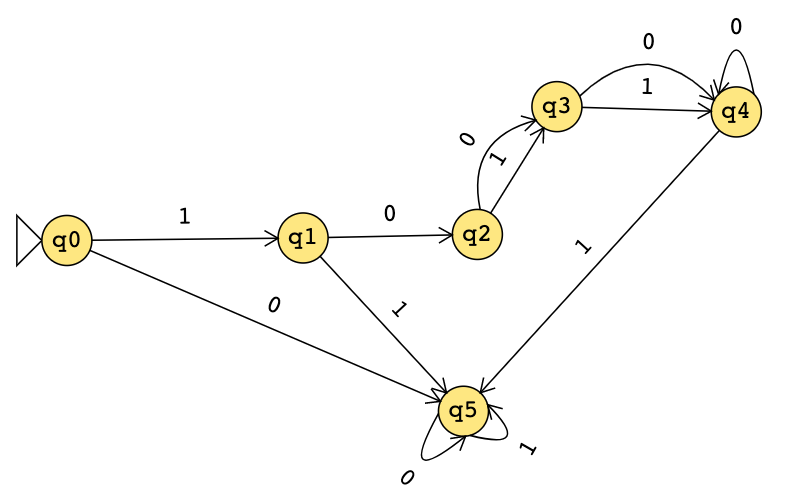
\includegraphics[width=3in]{../../resources/machines/hw1dfaCSE105Sp22.png}
   \caption{State diagram for DFA $C$}
\end{figure}

Suppose someone tells you that the formal definition of this DFA is 
\[
(Q, \Sigma, \delta, q_0, F) =  (\{ q0, q1, q2, q3, q4, q5 \}, \{0,1,2\}, \delta, q0, q0)
\]
where $\delta: Q \times \Sigma \to Q$ is given by 
\[
\hspace{-1in}\delta ( (q, 0) ) = \begin{cases}
q5 & \text{if $q=q0$} \\
qj & \text{if $q=qi$ and $i \in \{1,2,3\}$ and $j=i+1$} \\
q & \text{if $q \in \{q4,q5\}$} \\
\end{cases}  \qquad \delta ( (q, 1) ) = \begin{cases}
    q1 & \text{if $q=q0$} \\
    q5 & \text{if $q \in \{q1,q4,q5\}$} \\
    \delta( (q,0) ) & \text{if $q=q2$ or $q=q3$} \\
    \end{cases}
\]
\begin{enumerate}
\item Confirm that this formal description is correct (in that it is consistent with the 
state diagram), or fix any and all mistakes in it.
In your solution, explicitly address whether the description of the set of states is correct, whether the 
description of the alphabet is correct, 
whether the description of the transition function is correct, 
whether the description of the start state is correct, and whether 
the description of the accept states is correct, and why.

\item Modify the set of accept states of this state diagram to get a different DFA 
(with the same set of states, alphabet, start state, and transition function) 
that recognizes an infinite language. Your solution should include the 
diagram of this new DFA and an explanation of why the language it recognizes
is infinite.
\end{enumerate}


\item ({\it Graded for fair effort completeness})
Which of the following are valid descriptions using the terminology we have used in 
class and in the book so far? For those that aren't, explain what's wrong. For those that are, 
give an example of what's being described.
\begin{enumerate}
\item A finite automaton accepts a regular expression.
\item The language described by a regular expression is a finite automaton.
\item The empty string is the language of some regular expression.
\item A string of length one uses one symbol from the alphabet.
\item The input string runs a finite automaton.
\end{enumerate}


\end{enumerate}
\newpage

\title{HW2 : Regular Languages and Automata Constructions}
\date{Due: : 4/14/22 at 5pm (no penalty late submission until 8am next morning), via Gradescope}


\maketitle
\thispagestyle{fancy}


{\bf In this assignment,}

You will practice designing multiple representations of regular languages
and working with general constructions of automata to demonstrate the 
richness of the class of regular languages.

{\bf Resources}: To review the topics you are working with 
for this assignment, see the class material from  Week 1 and the start of Week 2.
We will post frequently asked questions and our answers to them in a 
pinned Piazza post.

{\bf Reading and extra practice problems}: Sipser Section 1.1, 1.2, 1.3.
Chapter 1 exercises 1.4, 1.5, 1.6, 1.7, 1.8, 1.9, 1.10, 1.11, 1.12, 1.14, 1.15, 1.16, 1.17, 1.19, 1.20, 1.21, 1.22.

{\bf Key Concepts}: Regular expressions, language described by a regular expression, deterministic finite automata (DFAs), 
regular languages, closure of the class of regular languages under certain operations, 
nondeterministic finite automata (NFA).


\instructions

You will submit this assignment via Gradescope
(\href{https://www.gradescope.com}{https://www.gradescope.com}) 
in the assignment called ``HW2CSE105Sp22''.

{\bf Assigned questions}


\begin{enumerate}
\item ({\it Graded for correctness}\footnote{This means your solution will be
evaluated not only on the correctness of your answers, but on your ability to 
present your ideas clearly and logically. You should explain how you arrived at 
your conclusions, using 
mathematically sound reasoning. Whether you use formal proof techniques or 
write a more informal argument for why 
something is true, your answers should always be well-supported. Your goal 
should be to convince the reader that 
your results and methods are sound.}) Over the alphabet $\{a,b\}$, consider the language
\[
    L = \{ w \in \{a,b\}^* \mid (ab \textrm{ is a substring of $w$}) \land (ba \textrm{ is a substring of $w$})
    \land (w \textrm{ starts with } a)\}
\]
In this question, you will use two different approaches to proving that this language is 
regular by building (different) DFA that recognize this language.
\begin{enumerate}
    \item Design a DFA recognizing the language $\{ w \in \{a,b\}^* \mid ab \textrm{ is a substring of $w$}\}$
    and a DFA recognizing the language $\{ w \in \{a,b\}^* \mid ba \textrm{ is a substring of $w$}\}$
    and a third DFA recognizing the language $\{ w \in \{a,b\}^* \mid w \textrm{ starts with } a\}$. Then, 
    use the construction we discussed in class to combine these DFA to get a DFA that recognizes
    $L$. A complete solution will include the (clearly labelled) state diagrams for each 
    of the three building-block DFAs, along with a description of the result of combining these DFAs that includes
    the formal definition of the resulting DFA and 
    at the least the part of the state diagram that includes the start state, all the outgoing edges
    from the start state, and specifies
    how many states the full DFA will have.
    \item Rewrite the language $L$ in a simpler form and use this simpler form to design a DFA with at most
    $5$ states that recognizes $L$. A complete solution will include the complete state diagram 
    of this DFA and a justification for why the DFA recognizes $L$.
\end{enumerate}

\item  To safeguard the privacy or security of a network, some software filters
the IP addresses that are allowed to send content to computers on the network. Each IP address
can be broken into parts that represent the source host of incoming traffic, including geographic data.
As a result, software needs to be designed to recognize whether certain substrings (representing
permitted hosts) are present (if the hosts are permitted to send data) and whether others
are absent (if those hosts are blocked from sending data).

In this question, you'll design ways to detect these patterns in strings.

\begin{enumerate}
    \item ({\it Graded for correctness})
    Over the alphabet $\{0,1,2,3,4,5,6,7,8,9\}$ design a DFA that accepts each and only strings
    that have $384$ or $116$ as a substring. Your DFA should have {\bf no more than $8$ states}.
    A complete solution will include the state diagram of your DFA and a brief justification of
    your construction by explaining the role each state plays in the machine. {\it Note: you may 
    include the formal definition of your DFA, but this is not required.} 
    \item ({\it Graded for correctness})
    Now suppose the network administrators want to block traffic from IP addresses
    that have been associated with spammers. Over the alphabet~$\{0,1,2,3,4,5,6,7,8,9\}$, 
    design an NFA with at most $5$ states that accepts each and only strings
    that do not have the substring $384$ and do not have the substring $116$. 
    A complete solution will include the state diagram of your NFA and a brief justification 
    of your construction by explaining the role each state plays in the machine.
    \item ({\it Graded for fair effort completeness}\footnote{This means 
    you will get full credit so long as your submission demonstrates honest 
    effort to answer the question. You will not be penalized for incorrect answers. 
    To demonstrate your honest effort in answering the question, we ask that you 
    include your attempt to answer *each* part of the question. If you get stuck 
    with your attempt, you can still demonstrate your effort by explaining where 
    you got stuck and what you did to try to get unstuck.})
    Give a regular expression that describes the set of strings over 
    the alphabet $\{0,1,2,3,4,5,6,7,8,9\}$ that have $384$ as a substring and give
    a (different) regular expression that describes the set of strings over
    the alphabet $\{0,1,2,3,4,5,6,7,8,9\}$ that do not have $384$ as a substring. Briefly justify
    why each of your regular expression works.
\end{enumerate}

\item In this question, you'll practice working with formal general constructions
for DFAs and translating between state diagrams and formal definitions.
Consider the following
construction in the 
textbook for Chapter 1 Problem 34, which we include here for reference: 
``Let $B$ and $C$ be languages over $\Sigma = \{ 0,1\}$. Define
\[
B \overset{1}{\leftarrow} C= \{ w \in B ~\mid~\textrm{ for some $y \in C$, strings $w$ and $y$ contain equal 
numbers of $1$s }\}
\]
The class of regular languages is shown to be closed under the $\overset{1}{\leftarrow}$ operation
using the construction: Let $M_B = (Q_B, \Sigma, \delta_B, q_B, F_B)$ and $M_C = ( Q_C, \Sigma, \delta_C, q_C, F_C)$ be DFAs recognizing the languages $B$ and $C$, respectively.  We will now construct NFA
$M = (Q, \Sigma, \delta, q_0, F)$ that recognizes $B \overset{1}{\leftarrow} C$ as follows.  To decide
whether its input $w$ is in $B \overset{1}{\leftarrow} C$, the machine $M$ checks that $w \in B$, and 
in parallel nondeterministically guesses a string $y$ that contains the same number of $1$s as 
contained in $w$ and checks that $y \in C$.
\begin{itemize}
\item[{\bf 1.}] $Q = Q_B \times Q_C$
\item[{\bf 2.}] For $(q,r) \in Q$ and $a \in \Sigma_\varepsilon$, define
\[
\delta( ~((q,r), a)~) = \begin{cases}
\{ (\delta_B(q,0) , r ) \}  \qquad&\textrm{if } a = 0 \\
\{ (\delta_B( q,1) ,  \delta_C( r,1) ) \}  \qquad&\textrm{if } a = 1 \\
\{ (q, \delta_C( r,0 ))\}  \qquad&\textrm{if } a = \varepsilon\\
\end{cases}
\]
\item[{\bf 3.}] $q_0 = (q_B, q_C)$
\item[{\bf 4.}] $F = F_B \times F_C$~~~."
\end{itemize}

\begin{enumerate}
\item ({\it Graded for correctness}) Illustrate this construction by defining specific example DFAs $M_B$ and $M_C$ and including 
their state diagrams in your submission.   Choose $M_B$ to have four states and $M_C$
to have two states, and make sure that every state in each state diagram is reachable from the start state
of that machine.
Apply the construction above to create the NFA $M$  and include its state diagram in your submission.
{\it Note: you may 
 include the formal definition of your DFAs and NFA, but this is not required.} 

{\it Hint: Confirm that you have specified every required piece of the state diagram for $M$. E.g., 
label the states consistently with the construction, indicate the start arrow, specify each
accepting state, and include all required transitions.}

\item ({\it Graded for fair effort completeness})  Describe the sets recognized by each of the 
machines you used in part (a): $M_B, M_C, M$.
If possible, give an example of a string that is in $B$ and in $B \overset{1}{\leftarrow} C$
and an example of a string that is in $B$ and not in $B \overset{1}{\leftarrow} C$. If any of these examples
do not exist, explain why not.
\end{enumerate}


\item ({\it Graded for fair effort completeness}) In last week's homework, 
we saw the definitions of two functions on the set of languages over $\{0,1\}$:
for $L$ a set of strings over the alphabet $\{0,1\}$, we can define the following associated sets
\[
LZ(L) = \{ 0^k w \mid w \in L, k \in \mathbb{Z}, k \geq 0 \}
\]
\[
TZ(L) = \{ w 0^k \mid w \in L, k \in \mathbb{Z}, k \geq 0 \}
\]
In this question, we'll develop a general construction that will prove
that if $L$ is regular then so are $LZ(L)$ and $TZ(L)$.

Consider an arbitrary regular
language $L$ over the alphabet $\Sigma = \{0,1\}$, and we are given that
$M = (Q, \Sigma, \delta, q_0, F)$ is a DFA over $\Sigma$ with $L(M) = L$.

\begin{enumerate}
\item Give the formal construction of an NFA $M'$ with $L(M') = LZ(L)$.  Briefly justify 
each parameter in the definition of  $M'$.
\item Apply your construction from part (a) when $L_{test} = L(M_{test})$, where the 
state diagram $M_{test}$ is below.  Submit the state diagram of the NFA that results.
If possible, give an example of a string that is in $LZ(L_{test})$ and one that is not; if either of these examples
do not exist, explain why not.

\item Give the formal construction of an NFA $N'$ with $L(N') = TZ(L)$.  Briefly justify 
each parameter in the definition of  $N'$. 
\item Apply your construction from part (c)  when $L_{test} = L(M_{test})$, where the 
state diagram $M_{test}$ is below.  Submit the state diagram of the NFA that results.
If possible, give an example of a string that is in $TZ(L_{test})$ and one that is not; if either of these examples
do not exist, explain why not.
\begin{figure}[h]
   \centering
   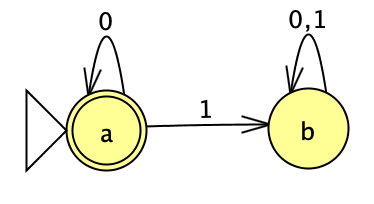
\includegraphics[width=2in]{../../resources/machines/MtestDFA.png}
   \caption{State diagram for DFA $M_{test}$}
\end{figure}
\end{enumerate}
{\it Caution}: Pay attention to the types of the components, especially
in the transition function.  You are given a DFA and are building an NFA.
\end{enumerate}
\newpage

\title{HW3 : Nonregular Languages and Pushdown Automata}
\date{Due: 4/28/22 at 5pm (no penalty late submission until 8am next morning), via Gradescope}


\maketitle
\thispagestyle{fancy}

{\bf In this assignment,}

You will practice distinguishing between regular and nonregular languages using both closure
arguments and the pumping lemma. You will also practice with the definition of pushdown automata.

{\bf Resources}: To review the topics you are working with 
for this assignment, see the class material from  Week 2 through Week 4.
We will post frequently asked questions and our answers to them in a 
pinned Piazza post.

{\bf Reading and extra practice problems}: Sipser Section 1.4, 2.2.
Chapter 1 exercises 1.29, 1.30. Chapter 1 problems 1.49, 1.50, 1.51. Chapter 2 exercises 2.5, 2.7.

{\bf Key Concepts}: Pumping lemma, pumping length, regular languages, 
nonregular languages, pushdown automata, stack.

\instructions

You will submit this assignment via Gradescope
(\href{https://www.gradescope.com}{https://www.gradescope.com}) 
in the assignment called ``HW3CSE105Sp22''.

\newpage
{\bf Assigned questions}
\begin{enumerate}
\item ({\it Graded for fair effort completeness}\footnote{This means 
you will get full credit so long as your submission demonstrates honest 
effort to answer the question. You will not be penalized for incorrect answers. 
To demonstrate your honest effort in answering the question, we ask that you 
include your attempt to answer *each* part of the question. If you get stuck 
with your attempt, you can still demonstrate your effort by explaining where 
you got stuck and what you did to try to get unstuck.})
Do the following for each of the following attempted ``proofs" that  a set is nonregular:
\begin{itemize}
\item[i] Find the (first and/or most significant) logical error in the ``proof" and describe why it's wrong.
\item[ii] Either prove that the set is actually regular (by finding a regular expression that describes it or 
a DFA/NFA that recognizes it, and justifying why) {\bf or} fix the proof so that it is logically sound.
\end{itemize}

\begin{enumerate}
\item The language $X_1 = \{ uw \mid \text{$u$ and
$w$ are strings over $\{0,1\}$ and have the same length} \}$.

\begin{quote}
``Proof" that $X_1$ is not regular using the Pumping Lemma: Let $p$ be 
an arbitrary positive integer. We will show that $p$ is not a pumping length for $X_1$. 

Choose $s$ to be the string $1^p 0^p$, which is in $X_1$ because
we can choose $u = 1^p$ and $w = 0^p$ which each have length $p$.
Since $s$ is in $X_1$ and has length greater than or equal to $p$, if $p$ were to be a
pumping length for $X_1$, $s$ ought to be pump'able. 
That is, there should be a way of dividing $s$ into parts $x,y,z$ where $s=xyz$,
$|y| >0$, $|xy| \leq p$, and for each $i \geq 0$, $xy^iz \in X_1$.
Suppose $x,y,z$ are such that $s = xyz$, $|y| > 0$ and $|xy| \leq p$.
Since the first $p$ letters of $s$ are all $1$ and $|xy| \leq p$, we know
that $x$ and $y$ are made up of all $1$s.  If we let $i=2$, we get 
a string $xy^iz$ that is not in $X_1$ because repeating $y$ twice adds $1$s to 
$u$ but not to $w$, and strings in $X_1$ are required to have $u$ and $w$ be the same
length. Thus, $s$ is not pumpable (even though it should have been if $p$ were to be a pumping length)
and so $p$ is not a pumping length for $X_1$.  Since $p$ was arbitrary, we have
demonstrated that $X_1$ has no pumping length.  By the Pumping Lemma, this implies that 
$X_1$ is nonregular.
\end{quote}


\item The language $X_2 = \{ u0w \mid \text{$u$ and
$w$ are strings over $\{0,1\}$ and have the same length} \}$.

\begin{quote}
``Proof" that $X_2$ is not regular using the Pumping Lemma: Let $p$ be 
an arbitrary positive integer. We will show that $p$ is not a pumping length for $X_2$. 

Choose $s$ to be the string $1^{p} 0^{p+1}$, which is in $X_2$ because
we can choose $u = 1^p$ and $w = 0^p$ which each have length $p$.
Since $s$ is in $X_2$ and has length greater than or equal to $p$, if $p$ were to be a
pumping length for $X_2$, $s$ ought to be pump'able. 
That is, there should be a way of dividing $s$ into parts $x,y,z$ where $s=xyz$,
$|y| >0$, $|xy| \leq p$, and for each $i \geq 0$, $xy^iz \in X_2$.
When $x = \varepsilon$ and $y = 1^{p}$ and $z = 0^{p+1}$,
we have satisfied that $s = xyz$, $|y| > 0$ (because $p$ is positive) and $|xy| \leq p$.
If we let $i=2$, we get 
the string $xy^iz = 1^{2p}0^{p+1}$ that is not in $X_2$ because its middle symbol is a $1$, not a $0$. 
Thus, $s$ is not pumpable (even though it should have been if $p$ were to be a pumping length)
and so $p$ is not a pumping length for $X_2$.  Since $p$ was arbitrary, we have
demonstrated that $X_2$ has no pumping length.  By the Pumping Lemma, this implies that 
$X_2$ is nonregular.
\end{quote}
\end{enumerate}

\item ({\it Graded for correctness}\footnote{This means your solution will be
evaluated not only on the correctness of your answers, but on your ability to 
present your ideas clearly and logically. You should explain how you arrived at 
your conclusions, using  mathematically sound reasoning. Whether you use formal proof techniques or 
write a more informal argument for why 
something is true, your answers should always be well-supported. Your goal 
should be to convince the reader that 
your results and methods are sound.}) Give an example of a language
over the alphabet $\{a,b,c\}$ that has cardinality $2$ and for which $4$ is a pumping length
and $3$ is not a pumping length.  A complete solution will give a clear and precise
description of the language, a justification for why $4$ is a pumping length, and a 
justification for why $3$ is not a pumping length.

\item  ({\it Graded for fair effort completeness})
Prove or disprove each of the following statements. (In other words, 
decide whether each statement is true or false and justify your decision.)
Fix $\Sigma$ an arbitrary (but unknown) alphabet.

\begin{enumerate}
\item If a language $L$ over $\Sigma$ is nonregular then its complement $\overline{L}$ is regular.
\item Each nonregular language over $\Sigma$ is infinite.
\item For each $w \in \Sigma^*$, there is a regular language $L_{w}$ such that $w \in L_{w}$.
\item For each $w \in \Sigma^*$, there is a nonregular language $L_{w}$ such that $w \in L_{w}$.
\item If a language over $\Sigma$ is recognized by a PDA then it is nonregular.
\end{enumerate}

\item ({\it Graded for correctness}) 
In the first week's homework, 
we saw the definitions of two functions on the set of languages over $\{0,1\}$:
for $L$ a set of strings over the alphabet $\{0,1\}$, we can define the following associated sets
\[
LZ(L) = \{ 0^k w \mid w \in L, k \in \mathbb{Z}, k \geq 0 \}
\]
\[
TZ(L) = \{ w 0^k \mid w \in L, k \in \mathbb{Z}, k \geq 0 \}
\]
This week we'll just focus on $LZ(L)$. 
In class and in the reading so far, we've seen the following examples of nonregular languages:
\begin{multicols}{3}
\begin{center}
$\{ 0^n 1^n ~|~ n \geq 0 \}$
$$\{ 0^n 1^n ~|~ n \geq 2 \}$$
$$\{ 0^n 1^m ~|~  0 \leq n \leq m \}$$
$$\{ 0^n 1^m ~|~ 0 \leq m \leq n \}$$
$$\{ 0^n 1^{2n} ~|~ 0 \leq n \}$$
$$\{ 0^n 1^{n+1} ~|~ 0 \leq n \}$$
$$\{ 1^{n^2} ~|~ 0 \leq n \}$$
$$\{ 0^n 1^m 0^n ~|~n,m \geq 0\}$$
$$\{ w \in \{0,1\}^* ~|~w = w^R\}$$
$$\{ w w^R ~|~ w \in \{0,1\}^*\}$$
\end{center}
\end{multicols}

Use (some of) the sets above, along with any regular sets you would like, to 
prove or disprove the statement: ``The class of nonregular languages
is closed under the function $LZ$.''

A complete solution will include a precise description of whether
the statement is true or false, referring back to the definition of closure, 
the definition of the function $LZ$, and the definition of nonregularity.
You may use any claims we proved in class or that are proved in the textbook reading,
so long as you reference them clearly in your argument by referring to a specific page 
in the notes, timestamp of a video, or page in the book.

{\it Bonus; not for credit: extend this homework problem for $TZ(L)$ as well.}

\item Consider the PDA with input
alphabet $\Sigma = \{ 0, 1\}$ and stack alphabet $\Gamma = \{\$, X\}$ 
and the following state diagram

\begin{center}
    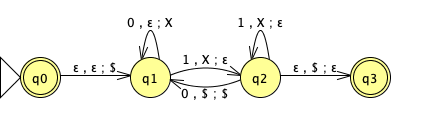
\includegraphics[width=3in]{../../resources/machines/hw3PDA.png}
\end{center}

\begin{enumerate}
\item ({\it Graded for correctness}) Specify an example string $w_1$ over $\Sigma$ that is accepted by this PDA, or explain why there is no such 
example. A complete solution will include either (1) a precise and clear 
description of your example  string and a precise and clear description of the accepting computation
of the PDA on this string (potentially using diagrams like those we used in class when tracing PDA
computations) or (2) a sufficiently
general and correct argument why there is no such example, referring back to the relevant definitions.
\item ({\it Graded for correctness}) Specify an example string $w_2$ over $\Sigma$ that is {\bf not} accepted by this PDA, 
or explain why there is no such 
example. A complete solution will include either (1) a precise and clear 
description of your example  string and a precise and clear description of all possible computations
of the PDA on this string (potentially using diagrams like those we used in class when tracing PDA
computations) to show that none of them are accepting or (2) a sufficiently
general and correct argument why there is no such example, referring back to the relevant definitions.
\item ({\it Graded for completeness}) Is the language recognized by this PDA regular or nonregular? You might 
find it useful to first write out this language in set notation.
\item ({\it Graded for completeness}) Modify the set of accept states of this state diagram to get a different PDA
(with the same set of states, input alphabet, stack alphabet, start state, and transition function) 
that recognizes an {\bf infinite  regular language}, if possible. A complete solution will include either (1) the 
diagram of this new PDA and an explanation of why the language it recognizes
is both infinite and regular, or (2) a sufficiently general and correct argument for why there is no way to choose 
the set of accept states to satisfy this requirement.
\end{enumerate}
\end{enumerate}
\newpage

\title{HW4: Context-free Languages and Turing Machines}
\date{Due: 5/5/22 at 5pm (no penalty late submission until 8am next morning), via Gradescope}


\maketitle
\thispagestyle{fancy}

{\bf In this assignment,}

You will practice designing and working with context-free grammars and 
pushdown automata. You will use general constructions to explore the class of context-free languages.
You will also practice with the formal definition of Turing machines.

{\bf Resources}: To review the topics you are working with 
for this assignment, see the class material from Weeks 4 and 5.
We will post frequently asked questions and our answers to them in a 
pinned Piazza post.

{\bf Reading and extra practice problems}: Sipser Sections 2.1, 2.2, 2.3 (partially).
Chapter 2 exercises 2.1, 2.2, 2.3, 2.4, 2.6, 2.9, 2.10, 2.11, 2.12, 2.13, 2.16, 2.17. Chapter 2 problem 2.30.
Chapter 3 exercises 3.1, 3.2.

{\bf Key Concepts}: Pushdown automata, stack, context-free grammar, derivations, context-free languages,
Turing machines, halting, looping.

\instructions

You will submit this assignment via Gradescope
(\href{https://www.gradescope.com}{https://www.gradescope.com}) 
in the assignment called ``HW4CSE105Sp22''.

\newpage
{\bf Assigned questions}
\begin{enumerate}
    \item For this question, we are working over the fixed alphabet $\{a,b,c\}$.

    \begin{enumerate}
        \item ({\it Graded for fair effort completeness}\footnote{This means 
        you will get full credit so long as your submission demonstrates honest 
        effort to answer the question. You will not be penalized for incorrect answers. 
        To demonstrate your honest effort in answering the question, we ask that you 
        include your attempt to answer *each* part of the question. If you get stuck 
        with your attempt, you can still demonstrate your effort by explaining where 
        you got stuck and what you did to try to get unstuck.})

    Consider the PDA over this alphabet with state diagram
        \begin{center}
        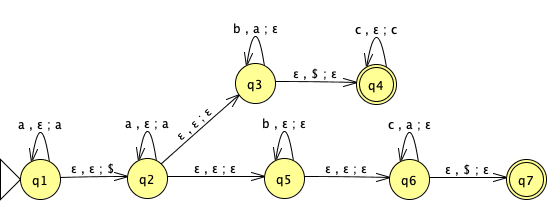
\includegraphics[width=4in]{../../resources/machines/hw4PDA.png}
        \end{center}

    Give an informal description of this PDA and describe the language it recognizes using 
    set builder notation.

    {\it Hint:} Compare the PDA with the machine in Example 2.16 and Figure 2.17 
    of the textbook (page 116), which recognizes 
    the language $\{a^i b^j c^k \mid i,j,k \geq 0 \textrm{ and } i=j \textrm{ or } i=k\}$ and 
    identify the main differences. 

    \item  ({\it Graded for correctness}\footnote{This means your solution will be
    evaluated not only on the correctness of your answers, but on your ability to 
    present your ideas clearly and logically. You should explain how you arrived at 
    your conclusions, using  mathematically sound reasoning. Whether you use formal proof techniques or 
    write a more informal argument for why 
    something is true, your answers should always be well-supported. Your goal 
    should be to convince the reader that 
    your results and methods are sound.}) 

    Consider the CFG $(\{X, S, S_1, S_2, T, Y\}, \{a,b,c\}, R, X)$ where the set of rules $R$ has
    \begin{align*}
        X &\to aX \mid S \mid T \\
        S &\to S_1S_2 \\
        S_1 &\to aS_1 b \mid \varepsilon \\
        S_2 &\to cS_2 \mid \varepsilon\\
        T &\to aTc \mid Y \\
        Y &\to bY \mid \varepsilon
    \end{align*}

    For each of the following strings, either give a derivation in this grammar that proves the 
    string is in the language generated by the grammar, or explain why there is no such derivation.
    \begin{enumerate}
        \item $aaaa$
        \item $abbc$
        \item $aabb$
    \end{enumerate}
    
    \item ({\it Graded for correctness}) Modify the start variable of this context-free grammar to get a 
    different CFG
    (with the same set of variables, set of terminals, and set of rules)
    that generates an {\bf infinite  regular language}, if possible. A complete solution will include either (1) the 
    formal definition of this new CFG and an explanation of why the language it recognizes
    is both infinite and regular, or (2) a sufficiently general and correct argument for why there is no way to choose 
    the start variable to satisfy this requirement.
    \end{enumerate}

    \item ({\it Graded for correctness}) 
    In this question, you'll practice working with formal general constructions
    for PDAs and translating between state diagrams and formal definitions.

    Suppose 
    \[
    M = (Q, \Sigma, \Gamma, \delta, q_0, F)
    \]
    is a PDA.  We can define a new
PDA $N$ so that $L(M) = L(N)$ and $N$ is {\bf guaranteed to have an empty stack} at the 
end of any accepting computation. 
Informally, the construction is as follows: Add three new states $q_1', q_2', q_3'$ and one new
stack symbol $\#$.  
\begin{itemize}
\item One of the new states $q_1'$ will be the new {\bf start} state and it has a spontaneous transition to the old start state $q_0$ which pushes the new stack symbol $\#$ to the stack. 
\item The transitions between the old states are all the same.
\item From each of the old accept states, {\bf add} a spontaneous
transition (that doesn't modify the stack) to the second new state $q_2'$.  
\item In this state $q_2'$, pop all old stack
symbols from the stack without reading any input. 
\item When the new stack symbol $\#$ is on the top of the stack, transition to the third new state $q_3'$ and accept.
\end{itemize}
Assume $\{ q_1', q_2', q_3'\} \cap Q = \emptyset$ (otherwise, relabel 
some of the states in $Q$) and assume that $\# \notin \Gamma$ (otherwise, relabel this stack symbol 
in $\Gamma$).  Define $N$ to be
\[
N = ( Q \cup \{ q_1', q_2', q_3'\} , \Sigma, \Gamma \cup \{\#\}, \delta_N, q_1', \{q_3'\} )
\]
where 
$\delta_N : Q \cup \{ q_1', q_2', q_3'\}~~\times~~ \Sigma_\varepsilon ~~\times~~\Gamma_\varepsilon\cup \{\#\}
\to \mathcal{P}( Q \cup \{ q_1', q_2', q_3'\} ~~\times ~~\Gamma_\varepsilon\cup \{\#\})$  is defined as
\[
\delta_N ( ~(q, x, y)~) = \begin{cases}
\{ (q_0, \#) \} &\qquad \text{if $q = q_1'$, $x = \varepsilon$, $y = \varepsilon$} \\
\delta( ~(q, x, y)~)  & \qquad \text{if $q \in Q$, $x \in \Sigma$, $y \in \Gamma_\varepsilon$} \\
\delta( ~(q, x, y)~)  & \qquad \text{if $q \in Q$, $x=\varepsilon$, $y \in \Gamma$} \\
\delta( ~(q, x, y)~)  & \qquad \text{if $q \in Q  \setminus F$, $x=\varepsilon$, $y =\varepsilon$} \\
\delta( ~(q, x, y)~) \cup \{  (q_2', \varepsilon) \}  & \qquad \text{if $q \in F$, $x=\varepsilon$, $y =\varepsilon$} \\
\{ (q_2', \varepsilon)\} & \qquad \text{if $q = q_2'$, $x = \varepsilon$, $y \in  \Gamma$} \\
\{ (q_3', \varepsilon)\} & \qquad \text{if $q = q_2'$, $x = \varepsilon$, $y = \#$} \\
\emptyset & \qquad \text{otherwise}
\end{cases}
\]

\begin{enumerate}
\item ({\it Graded for correctness})
Illustrate this construction by considering the PDA $M$ over the input alphabet 
$\{a,b,c\}$
\begin{center}
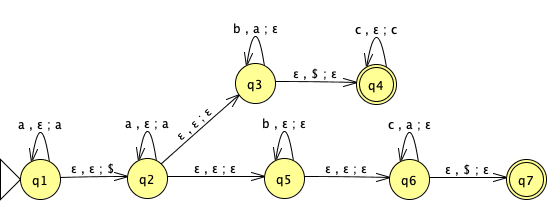
\includegraphics[width=5in]{../../resources/machines/hw4PDA.png}
\end{center}

and applying the construction above to create the related PDA $N$ and include its state diagram in your submission.
{\it Note: you may include the formal definition of your PDA, but this is not required.} 

\item ({\it Graded for correctness}) Pick a string of length $5$ over the alphabet of the PDA $M$ and use it to demonstrate
the difference in $M$ and in $N$ by 
\begin{itemize}
\item describing an accepting computation of $M$ on this string for which the stack is not empty
at the end of the computation, and
\item describing an accepting computation of $N$ on this string for which the stack is empty at the 
end of the computation.
\end{itemize}
In your descriptions of these computations, include both the sequence of states visited by the machine
as well as snapshots of the full contents of the stack at each step in the computation.  You may hand-draw
and scan these traces of the computations.

{\it Hint}: You will need to pick your example string wisely. It must be accepted by $M$ and 
there must be a computation of $M$ on your string which ends with a nonempty stack. Not all choices
of length $5$ strings work.

\end{enumerate}

\item  ({\it Graded for fair effort completeness})

Fix an arbitrary alphabet $\Sigma$. 
Prove that the class of context-free languages over $\Sigma$ is closed under concatenation in two ways:
\begin{enumerate}
    \item Prove that, for any languages $L_1, L_2$ over $\Sigma$, if there 
    are PDAs $M_1$ and $M_2$ such that $L_1 = L(M_1)$ and $L_2 = L(M_2)$, then there is 
    a PDA that recognizes $L_1 \circ L_2$.
    \item Prove that, for any languages $L_1, L_2$ over $\Sigma$, if there 
    are CFGs $G_1$ and $G_2$ such that $L_1 = L(G_1)$ and $L_2 = L(G_2)$, then there is 
    a CFG that generates $L_1 \circ L_2$.
\end{enumerate}


\item Consider the Turing machine $T$ over the input alphabet $\Sigma = \{0,1\}$ with  the state
    diagram below (the tape alphabet is $\Gamma = \{ 0,1,X,\square\}$).  
    Convention:  any missing transitions in the state diagram have value $(qrej,\square,R)$
    \begin{center}
    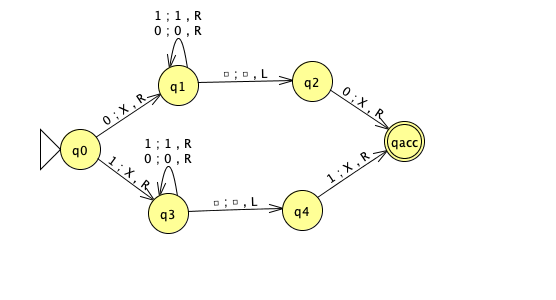
\includegraphics[width=3.5in]{../../resources/machines/hw4TM.png}
    \end{center}
    \begin{enumerate}

        \item ({\it Graded for correctness}) Specify an example string $w_1$ of length $4$ over 
        $\Sigma$ that is {\bf accepted} by this Turing machine, or explain why there is no such 
        example. A complete solution will include either (1) a precise and clear 
        description of your example  string and a precise and clear description of the accepting computation
        of the Turing machine on this string or (2) a sufficiently
        general and correct argument why there is no such example, referring back to the relevant definitions.
        
        To describe a computation of a Turing machine, include the contents of the 
        tape, the state of the machine, and the location of the read/write head at each step in the computation.
        
        {\it Hint:} In class we've drawn pictures to represent the configuration of the machine at each step 
        in a computation.  You may do so or you may choose to describe these configurations in words.
        
        \item ({\it Graded for correctness}) Specify an example string $w_2$ of length $3$ over $\Sigma$ 
        that is {\bf rejected} by this Turing machine
        or explain why there is no such 
        example. A complete solution will include either (1) a precise and clear 
        description of your example  string and a precise and clear description of the rejecting computation
        of the Turing machine on this string or (2) a sufficiently
        general and correct argument why there is no such example, referring back to the relevant definitions.

        \item ({\it Graded for correctness}) Specify an example string $w_3$ of length $2$ over $\Sigma$ 
        on which  the computation of this Turing machine {\bf loops}
        or explain why there is no such 
        example. A complete solution will include either (1) a precise and clear 
        description of your example  string and a precise and clear description of the looping (non-halting) 
        computation
        of the Turing machine on this string or (2) a sufficiently
        general and correct argument why there is no such example, referring back to the relevant definitions.

        \item ({\it Graded for fair effort completeness}) Write an implementation level description of 
        the Turing machine $T$.
\end{enumerate}

\end{enumerate}
\newpage

\title{HW5: Recognizability, Decidability, Undecidability, and Reductions}
\date{Due: 5/26/22 at 5pm (no penalty late submission until 8am next morning), via Gradescope}


\maketitle
\thispagestyle{fancy}

{\bf In this assignment,}

You will practice designing and working with Turing machines and their variants. 
You will use general constructions and specific machines to explore the classes of recognizable, 
decidable, and undecidable languages.
You will use computable functions to relate the difficult levels of languages via mapping reduction.

{\bf Resources}: To review the topics you are working with 
for this assignment, see the class material from Weeks 6, 7, 8.
We will post frequently asked questions and our answers to them in a 
pinned Piazza post.

{\bf Reading and extra practice problems}: Chapter 4 exercises 4.1, 4.3, 4.4., 4.5. 
Chapter 4 Problems 4.29, 4.30, 4.32.  Chapter 5 exercises 5.4, 5.5, 
5.6, 5.7. Chapter 5 problems 5.10, 5.11, 5.16, 5.18.

{\bf Key Concepts}: Formal definitions of Turing machines, computations of Turing machines,
halting computations, implementation-level descriptions of Turing machines, high-level descriptions
of Turing machines, recognizable languages, decidable languages, variants of Turing machines,
enumerators, nondeterministic Turing machines, Church-Turing thesis,
 computational problems, diagonalization, undecidability, unrecognizability, 
computable function, mapping reduction.

\instructions

You will submit this assignment via Gradescope
(\href{https://www.gradescope.com}{https://www.gradescope.com}) 
in the assignment called ``HW5CSE105Sp22''.

\newpage
{\bf Assigned questions}
\begin{enumerate}
    \item ({\it Graded for correctness}\footnote{This means your solution will be
    evaluated not only on the correctness of your answers, but on your ability to 
    present your ideas clearly and logically. You should explain how you arrived at 
    your conclusions, using  mathematically sound reasoning. Whether you use formal proof techniques or 
    write a more informal argument for why 
    something is true, your answers should always be well-supported. Your goal 
    should be to convince the reader that 
    your results and methods are sound.}) 
    \begin{enumerate}
        \item Give an example of a decidable language $L_1$ whose complement is also decidable.
        A complete solution will include either (1) a precise definition of the example language $L_1$ and 
        an explanation of why it is decidable and why its complement is decidable, or 
        (2) a sufficiently general and correct argument for why there is no way to choose 
        an example language to satisfy this requirement. All justifications and arguments should
        connect to the relevant definitions and the specific concepts being discussed.
        \item Give an example of a decidable language $L_2$ and a Turing machine $M_2$ such that
        $L(M_2) = L_2$ but $M_2$ does not decide $L_2$.  A complete solution will include either (1) precise
        definitions of $L_2$ and $M_2$ and justifications for why $L(M_2) = L_2$ and why $M_2$
        does not decide $L_2$, or (2) a sufficiently general and correct argument for why there is no way to choose 
        such a language and machine. For any machines you discuss, you can choose whether to use high-level descriptions,
        implementation level descriptions, or formal definitions. All justifications and arguments should
        connect to the relevant definitions and the specific concepts being discussed.
    \end{enumerate}
    \item ({\it Graded for fair effort completeness}\footnote{This means 
    you will get full credit so long as your submission demonstrates honest 
    effort to answer the question. You will not be penalized for incorrect answers. 
    To demonstrate your honest effort in answering the question, we ask that you 
    include your attempt to answer *each* part of the question. If you get stuck 
    with your attempt, you can still demonstrate your effort by explaining where 
    you got stuck and what you did to try to get unstuck.})

    Recall that a set $X$ is said to be {\bf closed} under an operation $OP$ if, for any elements in $X$, applying 
    $OP$ to them gives an element in $X$.  For example, the set of integers is closed under multiplication
    because if we take any two integers, their product is also an integer.
    
    Suppose $M_1$  and $M_2$ are Turing machines.  Consider the following high-level  
    descriptions of machines that give general constructions based on  $M_1$  and $M_2$.
    
    \begin{enumerate}
    \item Consider the  following construction of a nondeterministic  Turing  machine:
    \begin{quote}
    ``On  input $w$
    \begin{itemize}
    \item[1.] Nondeterministically  split $w$ into two pieces, i.e. choose  $x,y$  such that  $w =  xy$.
    \item[2.] Simulate running $M_1$ on  $x$.
    \item[3.] Simulate running $M_2$ on  $y$.
    \item[4.] If both simulations in steps 2 and 3 accept, accept."
    \end{itemize}
    \end{quote}
    
    Can  this construction  be  used  to prove that the class  of  Turing-recognizable languages is closed under 
    concatenation? Briefly  justify your  answer.
    
    \item Consider the  following construction of an enumerator: 
    \begin{quote}
    ``Without any input
    \begin{itemize}
    \item[1.] Build an enumerator $E_1$ that is equivalent to  $M_1$.
    \item[2.] Build an enumerator $E_2$ that is equivalent to  $M_2$.
    \item[3.] Start $E_1$ running and start $E_2$ running.
    \item[4.] Initialize a list of all strings that have been printed by $E_1$. Declare the variable $n_1$ to be the length of  this  list 
    (initially $n_1 = 0$).
    \item[5.] Initialize a list of all strings that have been printed 
    by $E_2$ so far.
    Declare the variable $n_2$ to be the length of  this  list (initially $n_2 = 0$).
    \item[6.] Every time a new string $x$ is printed by $E_1$: 
    \item[7.] \qquad Add this string to the list of strings printed by $E_1$ so far.
    \item[8.] \qquad Increment $n_1$ so it stores the current length of the list.
    \item[9.] \qquad For $j =  1 \ldots n_2$, 
    \item[10.] \qquad \qquad Let $w_j$ be the $j$th string in the list of strings printed  by  $E_2$
    \item[11.] \qquad \qquad Print $xw_j$.
    \item[12.] Every time a new string $y$ is printed by $E_2$: 
    \item[13.] \qquad Add this string to the list of strings printed by $E_2$ so far.
    \item[14.] \qquad Increment $n_2$ so it stores the current length of the list.
    \item[15.] \qquad For $i =  1 \ldots n_1$, 
    \item[16.] \qquad \qquad Let $u_i$ be the $i$th string in the list of strings printed  by  $E_1$
    \item[17.] \qquad \qquad Print $u_i y$."
    \end{itemize}
    \end{quote}
    
    Can this construction  be  used  to prove that the class  of  Turing-recognizable languages is closed under 
    concatenation? Briefly justify your  answer.
    
    \item Consider the following construction of a Turing machine:
    \begin{quote}
    ``On input $w$
    \begin{itemize}
    \item[1.] Let  $n = |w|$.
    \item[2.] Create a two dimensional array of strings  $s_{m,j}$ where $0 \leq m \leq n$ and  $0 \leq j \leq  1$.
    \item[3.] For each  $0 \leq m  \leq n$, initialize $s_{m,0}$ to be the prefix of  $w$ of length $m$ and $s_{m,1}$ to be
    the suffix  of $w$ of length  $n-m$.  In other words, $w= s_{m,0} s_{m,1}$  and $|s_{m,0}| = m$, $|s_{m,1}| =  n-m$.
    \item[4.] For $i = 1, 2, \ldots$
    \item[5.] \qquad For $k = 0, \ldots, i$
    \item[6.] \qquad \qquad  Run $M_1$  on $s_{\min{(k,n)},0}$ for (at most) $i$ steps.
    \item[7.] \qquad \qquad  Run $M_2$  on $s_{\min{(k,n)},1}$ for (at most) $i$ steps.
    \item[8.] \qquad \qquad If  both simulations  in steps 6 and 7 accept,  accept."
    \end{itemize}
    \end{quote}
    
    Can  this construction  be  used  to prove that the class  of  Turing-recognizable languages is closed under 
    concatenation? Briefly  justify your  answer.
    \end{enumerate}

    \item ({\it Graded for fair effort completeness}) 
    Recall that 
    \[
        A_{TM} =  \{ \langle M,  w \rangle \mid \text{$M$ is a  Turing machine, 
    $w$ is a string, and $w \in L(M)$} \}
    \]
     and 
    \[
         HALT_{TM} = \{ \langle M, w \rangle \mid \text{$M$ is a Turing machine,
    $w$ is a string, and $M$ halts on $w$}\}
    \]

    Consider the Turing machines below, with input alphabet $\Sigma = \{0,1\}$, tape alphabet 
    $\{0, 1, \textvisiblespace\}$, and state diagrams (with the usual conventions):
    \begin{center}
    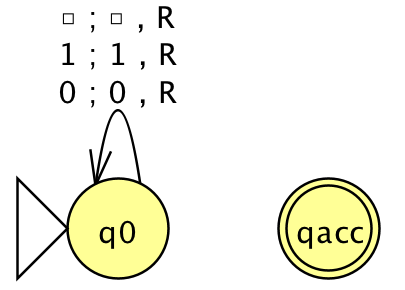
\includegraphics[width=1in]{../../resources/machines/Lect22TM1.png}\qquad\hfill \qquad
    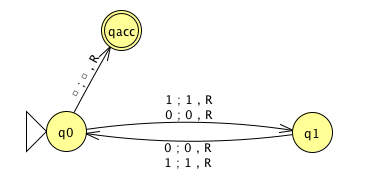
\includegraphics[width=2in]{../../resources/machines/Lect22TM2.png}
    \end{center}
    \begin{enumerate}
    \item Give an example string that is in both $A_{TM}$ and $HALT_{TM}$ and that is related to one of the 
    two Turing machines whose state diagrams are given above, or explain why there is no such string.
    \item  Give an example string that is in $A_{TM}$ and is not in $HALT_{TM}$ and that is related to one of the 
    two Turing machines whose state diagrams are given above, or explain why there is no such string.
    \item Give an example string that is not in $A_{TM}$ and is in $HALT_{TM}$ and that is related to one of the 
    two Turing machines whose state diagrams are given above, or explain why there is no such string.
    \end{enumerate}
    
    \item ({\it Graded for correctness}) Fix  $\Sigma = \{0,1\}$  for this question. 
    For each part below, you can choose sets from the  following list:  
    \[
    \emptyset, A_{TM}, \overline{A_{TM}}, HALT_{TM}, \overline{HALT_{TM}}, E_{TM}, \overline{E_{TM}}, 
    EQ_{TM}, \overline{EQ_{TM}}, \Sigma^*
    \]
    You may use each set from the list {\bf at most once} in the examples below.  In  particular, you can't choose
    $A =  B = C =  D = X = Y =  \Sigma^*$.

    
    \begin{enumerate}
    \item Find sets $A, B$ for which  the computable function
    \begin{align*}
    F &= \text{``On input $x$} \\
    &\text{1. Output $\langle 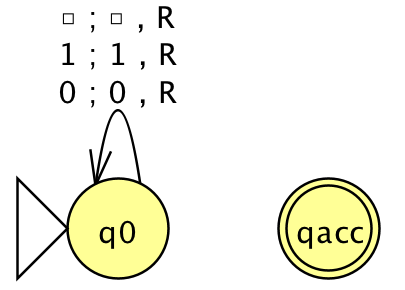
\includegraphics[width=0.5in]{../../resources/machines/Lect22TM1.png} , 00\rangle$."}
    \end{align*}
    
    witnesses the mapping reduction $A  \leq_m B$.
    Justify your  answer by  proving that, for all  strings  $x$, $x \in A $ iff  $F(x) \in B$.
    If no such sets exist, justify why not.
    
    \vfill
    
    \item Find sets $C, D$ for which  the computable function
    \begin{align*}
    G &= \text{``On input $x$} \\
    &\text{1. Check if $x = \langle M, w \rangle$ for $M$ a Turing machine and $w$ a string. If so, go to  step 3.}\\
    &\text{2. If not, output  $\langle 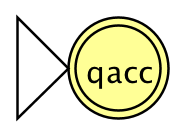
\includegraphics[width=0.5in]{../../resources/machines/hw5tm1.png},   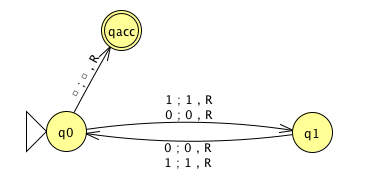
\includegraphics[width=1in]{../../resources/machines/Lect22TM2.png} \rangle$.}\\
    &\text{3. Construct the Turing machine $M'_x = $ ``On input $y$,} \\
    &\text{\qquad 1. If $y$ has a positive and odd length, reject.}\\
    &\text{\qquad 2. Else, if $y$ has a positive and even length, accept.}\\
    &\text{\qquad 3. Otherwise, run $M$ on $w$ and, if the computation halts, accept $y$."}\\
    &\text{4. Output  $\langle M'_x , 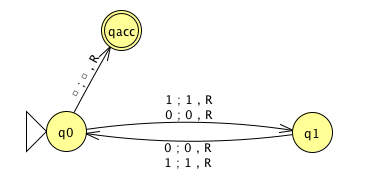
\includegraphics[width=1in]{../../resources/machines/Lect22TM2.png}\rangle$."}
    \end{align*}
    
    \vspace{-10pt}
    
    witnesses the mapping reduction $C  \leq_m D$.
    Justify your  answer by  proving that, for all  strings $x$, $x \in C $ iff  $G(x) \in D$.
    If no such sets exist, justify why not.

    
    \vfill
    
    \item Find sets $X, Y$ for which  the computable function
    \begin{align*}
    H &= \text{``On input $x$} \\
    &\text{1. Check if $x = \langle M, w \rangle$ for $M$ a Turing machine and $w$ a string. If so, go to  step 3.}\\
    &\text{2. If not, output  $\langle 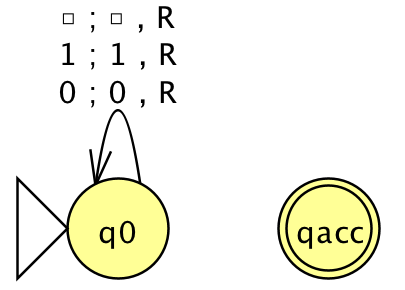
\includegraphics[width=1in]{../../resources/machines/hw5tm2.png}\rangle$.}\\
    &\text{3. Construct the Turing machine $M'_x = $ ``On input $y$,} \\
    &\text{\qquad 1. If $y \neq w$, reject.}\\
    &\text{\qquad 2. Otherwise, run $M$ on $w$.}\\
    &\text{\qquad 3. If $M$  accepts,  accept.  If  $M$ rejects, reject."} \\
    &\text{4. Output  $\langle M'_x \rangle$."}
    \end{align*}
    
    \vspace{-10pt}
    
    witnesses a mapping reduction $X \leq_m Y$. 
    Justify your  answer by  proving that, for all  strings $x$, $x \in X $ iff  $H(x) \in Y$.
    If no such sets exist, justify why not.
    
    \end{enumerate}
\end{enumerate}
\newpage

\title{Project}
\date{Part 1 due TBA; Part 2 due TBA; Part 3 due TBA}


\maketitle
\thispagestyle{fancy}
The project component of this class will be an opportunity for you to extend your 
work on assignments and explore applications of your choosing. 

{\it Why?}
TBA

{\it How?} During emergency remote instruction last academic year, we discovered
that video assessement and some open-ended personalized projects help ensure fairness
and can be less stressful for students than in-person midterm exams. Asynchronous project
submission also gives flexibility and allows more physical distancing.

Your videos: We will delete all the videos we receive from you after assigning final grades for the course, 
and they will be stored in a university-controlled Google Drive directory 
only accessible to the course staff during the quarter. 
Please send an email to the instructor (minnes@eng.ucsd.edu) if you have 
concerns about 
the video / screencast components of this project or cannot complete projects in this style for some reason.

You may produce screencasts with any software you choose. 
One option is to record yourself with Zoom; a tutorial on how to use Zoom to record a 
screencast (courtesy of Prof. Joe Politz)  is here: 

\url{https://drive.google.com/open?id=1KROMAQuTCk40zwrEFotlYSJJQdcG_GUU}.

The video that was produced from that recording session in Zoom is here:

\url{https://drive.google.com/open?id=1MxJN6CQcXqIbOekDYMxjh7mTt1TyRVMl}

\subsection*{What resources can you use?}
This project must be completed individually, without any help from other people, 
including the course staff (other than logistics support if you get stuck with screencast). 

You can use any of this quarter's CSE 20 offering (notes, readings, class videos, homework feedback). 
These resources should be more than enough. If you are struggling to get started and want to 
look elsewhere online, you must acknowledge this by listing and citing any resources you consult 
(even if you do not explicitly quote them). Link directly to them and include the name of the 
author / video creator and the reason you consulted this reference. The work you submit for 
the project needs to be your own. Again, you shouldn't need to look anywhere other 
than this quarter's material and doing so may result in definitions or notations 
that conflict with our norms in this class so think carefully before you go down this path.

The project has three parts. 
\begin{itemize}
    \item Part 1 of Project: due TBA
    \item Part 2 of Project: due TBA
    \item Part 3 of Project: due TBA
\end{itemize}

\newpage
\subsection*{Part 1: due TBA}
\subsubsection*{Written component}


\subsubsection*{Video component}
Presenting your reasoning and demonstrating it via screenshare are important 
skills that also show us a lot of your learning. Getting practice with this style of 
presentation is a good thing for you to learn in general and a rich way for us to assess your skills. 

Prepare a 3-5 minute screencast video that starts with 
your face and your student ID for a few seconds at the beginning, and introduce yourself audibly while on screen. 
You don't have to be on camera for the rest of the video, though it's fine if you are. 
We are looking for a brief confirmation that it's you creating the video and doing the work 
submitted for the project.

Then, explain your work in question 1 of the written component.
Discuss at least one potential mistake that someone solving 
a similar question should avoid (this could be a mistake you made while thinking about this 
problem or something you anticipate a classmate might struggle with); explain why the 
mistake is wrong and how to fix it.
 
TBA

Gradescope online submission

\subsubsection*{Checklist (this is how we will grade Part 1 of the project)}
\begin{itemize}
\item Question 1: TBA
\end{itemize}

\newpage
\subsection*{Part 2: due TBA}
\subsubsection*{Written component}
\begin{enumerate}
\item In this part of the project, you will select one question from one of the review quizzes 
TBA to revisit. 
Include the problem statement, why you picked this question (e.g. what is interesting about it, 
what is hard about it, or why you wanted to take a second look at it), and your solution. 
    \begin{itemize}
        \item Question selection: you can pick any {\bf one question} listed in the Review 
        sections of the relevant notes documents, and you must address all of its parts.
        \item For each part of your chosen question: prepare a complete solution 
        (you can use the homework solutions we post for guidance about the style). 
        Your submission will be evaluated not only on the correctness of your answers, 
        but on your ability to present your ideas clearly and logically. 
        You should explain how you arrived at your conclusions, using mathematically 
        sound reasoning. Your goal should be to convince the reader that your results 
        and methods are sound. Imagine you are preparing these solutions for someone else 
        taking CSE 20 who missed that week and is ``catching up".
    \end{itemize}
\item In this part of the project, you'll TBA

\end{enumerate}

\subsubsection*{Video component}

Presenting your reasoning and demonstrating it via screenshare are important skills that 
also show us a lot of your learning. Getting practice with this style of presentation 
is a good thing for you to learn in general and a rich way for us to assess your skills. 

Prepare a 3-5 minute screencast video explaining your work in question 1 of the written component.
During your solution presentation, point out at least one potential mistake that someone 
solving a similar question should avoid (this could be a mistake you made while thinking 
about this problem or something you anticipate a classmate might struggle with); 
explain why the mistake is wrong and how to fix it. 

You do not need to include complete details of every part of your solution. 
It is up to you to choose what is most important so that you can stick to the 
timing guidelines and still have time to include discussing potential mistakes.

Include your face and your student ID (we'd like a photo ID that includes your name 
and picture if possible) for a few seconds at the beginning, and introduce yourself 
audibly while on screen. You don't have to be on camera the whole time, though it's fine 
if you are. We are looking for a brief confirmation that it's you creating the 
video/doing the work attached to the video.


Then, explain your work in question 1 of the written component.
Discuss at least one potential mistake that someone solving 
a similar question should avoid (this could be a mistake you made while thinking about this 
problem or something you anticipate a classmate might struggle with); explain why the 
mistake is wrong and how to fix it.
 
TBA

\subsubsection*{Checklist (this is how we will grade Part 2 of the project)}
\begin{itemize}
\item Question 1
    \begin{itemize}
        \item Selected review quiz question is labelled clearly, including the day 
        it belongs to and the statement of the question.
        \item Solution is complete: it addresses each part of the review quiz question selected.
        \item Solution is correct: it clearly and correctly justifies the correct answer 
        for each part of the question. You are welcome to check your answers with the 
        Gradescope autograder (we will be reopening the review quizzes for this purpose). 
        We will evaluate your submissions for the quality of your justification.
    \end{itemize}
\item Question 2
    \begin{itemize}
        \item A key lesson from each of the three references is stated clearly and 
        is relevant to the message of the articles. Supporting explanations are included.
        \item A specific example of an instance where using computers/ CS *caused* an error is described.
        \item A specific example of an instance where using computers/ CS helped *avoid* an error is described.
        \item Lesson(s) are drawn from the previous experiences.
        \item Specific strategies for increasing confidence in computation are described and justified.
    \end{itemize}
    \item Video
    \begin{itemize}
        \item Video loads correctly and is between 3 and 5 minutes. It includes your face and your student ID, 
        and you introduce yourself audibly while on screen.
        \item Video presents your solution for Question 1.
        \item A potential mistake is presented and discussed.
    \end{itemize}
\end{itemize}

\newpage
\subsection*{Part 3: due TBA}
\subsubsection*{Written component}
\begin{enumerate}
    \item In this part of the project, you will TBA
\end{enumerate}

\subsubsection*{Video component}
Presenting your reasoning and demonstrating it via screenshare are important skills that 
also show us a lot of your learning. Getting practice with this style of presentation 
is a good thing for you to learn in general and a rich way for us to assess your skills. 

Prepare a 3-5 minute screencast video explaining your work in question 1 parts (c) and (d)
of the written component (i.e. the negation and proof).
During your solution presentation, point out at least one potential mistake that someone 
solving a similar question should avoid (this could be a mistake you made while thinking 
about this problem or something you anticipate a classmate might struggle with); 
explain why the mistake is wrong and how to fix it. 

You do not need to include complete details of every part of your solution to these parts. 
It is up to you to choose what is most important so that you can stick to the 
timing guidelines and still have time to include discussing potential mistakes.

Include your face and your student ID (we'd like a photo ID that includes your name 
and picture if possible) for a few seconds at the beginning, and introduce yourself 
audibly while on screen. You don't have to be on camera the whole time, though it's fine 
if you are. We are looking for a brief confirmation that it's you creating the 
video/doing the work attached to the video.

Then, explain your work in question 1 of the written component.
Discuss at least one potential mistake that someone solving 
a similar question should avoid (this could be a mistake you made while thinking about this 
problem or something you anticipate a classmate might struggle with); explain why the 
mistake is wrong and how to fix it.
 
TBA


\subsubsection*{Checklist (this is how we will grade Part 3 of the project)}
\begin{itemize}
    \item Question 1 TBA
\item Video
    \begin{itemize}
        \item Video loads correctly and is between 3 and 5 minutes. It includes your face and your student ID, 
        and you introduce yourself audibly while on screen.
        \item Video presents your solution for Question 1 parts (c) and (d).
        \item A potential mistake is presented and discussed.
    \end{itemize}
\end{itemize}
\newpage

\title{Project - CSE 105 Spring 2022}
\date{Part 2 due 5/19/22 at 5pm (no penalty late submission until 8am next day)}


\maketitle
\thispagestyle{fancy}

\vspace{-30pt}

 The project component of this class will be an opportunity for you to extend your work on 
 assignments and explore applications of your choosing. 
 
 Why?  To go deeper and explore the material from Theory of Computation and how it relates to 
 other aspects of CS and beyond. 
 
 How?  During emergency remote instruction last academic year, we discovered that video 
 assessment and some open-ended personalized projects help ensure fairness and can be less 
 stressful for students than in-person midterm exams. Asynchronous project submission also 
 gives flexibility and allows more physical distancing. 
 
 {\bf Your videos}: We will delete all the videos we receive from you after assigning final grades for 
 the course, and they will be stored in a university-controlled Google Drive directory only 
 accessible to the course staff during the quarter. Please send an email to the instructor 
 (minnes@eng.ucsd.edu) if you have concerns about the video / screencast components of this 
 project or cannot complete projects in this style for some reason. 
 
 You may produce screencasts with any software you choose. One option is to record yourself 
 with Zoom; a tutorial on how to use Zoom to record a screencast (courtesy of Prof. Joe Politz) is 
 here: \href{https://drive.google.com/open?id=1KROMAQuTCk40zwrEFotlYSJJQdcG_GUU}{Tutorial URL}
 The video that was produced from that recording session in Zoom is here:
 \href{{https://drive.google.com/open?id=1MxJN6CQcXqIbOekDYMxjh7mTt1TyRVMl}}{Video produced in tutorial} .
 
 {\bf What resources can you use? }
 This project must be completed individually, without any help from other people, 
 including the course staff (other than logistics support if you get stuck with screencast). 
 You can use any of this quarter’s CSE 105 offering (notes, readings, class videos, 
 supplementary videos, homework feedback). You may additionally search online to respond to 
 project parts that explicitly ask you to do so, and you must  cite all resources (online or offline) 
 that you consult as part of this search. Link directly to the resource and include the name of the 
 author / video creator and the reason you consulted this reference. The work you submit for the 
 project needs to be your own. 
 
The written portion of the project is expected to be clearly legible, and should preferably be typed.

 \newpage
 \section{Tasks for Project Part 2}


 \subsection{Task 1: Explain a review quiz question (Written)}
	
	\begin{enumerate}
		\item Select one question from one of the review quizzes from 4/15/22 (Friday of Week 3) to 4/29/22  (Friday of Week 5) to revisit. Include the problem description, why you picked this question (e.g. what is interesting about it, what is hard about it, or why you wanted to take a second look at it), and your solution. Question selection: you can pick any one question listed in the Gradescope review quizzes, and you must address  all  of its parts. 
 		\item For each part of your chosen question: prepare a complete solution (you can use the homework solutions we post for guidance about the style). Your submission will be evaluated not only on the correctness of your answers, but on your ability to present your ideas clearly and logically. You should explain how you arrived at your conclusions, using mathematically sound reasoning. Your goal should be to convince the reader that your results and methods are sound. Imagine you are preparing these solutions for someone else taking CSE 105 who missed that week and is “catching up”
 
 		\item Include at least 2 potential mistakes that a student may have made while attempting to solve the quiz problem that you selected. Explain why the reasoning behind these mistakes is flawed so that a student reading this may learn from these mistakes. It’s a good idea to include mistakes that you made when you first tried to solve this problem!	
	\end{enumerate}
	
	{\bf Style guidelines}: your written submission for Task 1 should clearly label the three parts:
	{\it Question Selection}, {\it Solution},  and {\it Potential Mistakes}.

\newpage
\subsection{Task 2: Closure of the Collection of Regular Languages}
	
	For this task, we fix $\Sigma = \{0,1\}$. Recall that the composition of two 
	functions $f$ and $g$ is denoted $f \circ g$, which can also be written as $f(g(x))$, and is the 
	result of first applying the function $g$ to the input $x$ (producing $g(x)$), and then applying $f$ to $g(x)$. 
	Below are some functions with domain and codomain $\mathcal{P}(\Sigma^*)$; that is, they 
	each take in a language over $\Sigma$
	and output a language over $\Sigma$. 
	
	\begin{align*}
		TZ(L) &= \{ w0^k \mid w \in L, k \geq 0 \}\\
		R(L) &= \{ w \mid w^R \in L\} \textrm{(where $w^R$ is reversing $w$, e.g. $(100)^R = 001$)}\\
		E(L) &= \{ w \mid w \in L, \textrm{ the length of $w$ is even} \} \\
		T(L) &= \{ w \mid w \in L, \textrm{ the length of $w$ is a multiple of } 3 \}\\
		EQ(L) &= \{ w^k1^k \mid k \geq 0, w \in L \} \textrm{(where $w^k$ is concatenating $w$ with itself $k$ times, e.g. $(100)^2 = 100100$)}\\
		LT(L) &= \{ w^k1^j \mid 0 \leq k < j , w \in L \}\\
		EQ2(L) &= \{ w^kx^k \mid k \geq 0, w \in L, x \in L \}
	\end{align*}

	For example $(TZ \circ R)(L) = TZ(R(L)) = \{ w^R 0^k | w \in L, k \geq 0\}$.

	
	\begin{enumerate}
		\item Choose two functions from the above list so that their 
		composition, $h$, is such that the collection of regular languages over $\Sigma$ is closed under $h$.
		
		\begin{enumerate}
			\item Provide a clear and complete definition of  your function $h$.
			A complete solution will clearly specify the two functions you chose to compose, 
			the order in which $h$ applies them, and a general description of what the function $h$ does using set builder
			descriptions and/or English prose.
			{\bf Note:} You do not need to apply $h$ to a language in this step, you only need to define $h$.
			\item Prove that the collection of regular languages over $\Sigma$ is 
			closed under $h$ by writing out the following argument in detail: 
			Consider an arbitrary regular language $L$ over the alphabet $\Sigma = \{0, 1\}$.
			Since it is regular, it is recognized by a DFA and let $M = (Q, \Sigma, \delta, q_0, F)$ 
			be such a DFA over $\Sigma$ with $L(M) = L$. 
			Give the formal construction of an NFA $N$ with $L(N) = h(L)$ for your function $h$.
			Briefly justify this construction by tracing the computations of $N$ and/or referencing constructions
			we discussed in class and in the book. In particular, explain the role of each parameter in the definition of $N$ in 
			the construction.
		\end{enumerate}
		
		\item Choose two functions from the above list so that their composition, $h'$, 
		is such that the collection of regular languages over $\Sigma$ is {\bf not} closed under $h'$. 
		{\it Note the functions you choose for this part may or may not overlap with those from the previous part; it's up to you to decide.}
		
		\begin{enumerate}
			\item Provide a clear and complete definition of  your function $h'$.
			A complete solution will clearly specify the two functions you chose to compose, 
			the order in which $h'$ applies them, and a general description of what 
			the function $h'$ does using set builder
			descriptions and/or English prose.			
			\item Give a witness language $L$ that can be used to prove that the class of regular
			languages over $\Sigma$ is not closed under $h'$. To do so: 
			(1) clearly define a language $L$ over $\Sigma$, (2) prove that $L$ is regular, and (3) prove that $h'(L)$ is not regular.
			You may use results proved in class and / or the relevant sections in the textbook as part of your proofs 
			if you would like, but you must label these results and provide references to the day we discussed them and/or the 
			page number in the book.
		\end{enumerate}
	\end{enumerate}
		
\subsection{Task 3: Implementation examples and Video}
 With the introduction of PDAs, our models of computation begin to approach the power that 
 modern day computers have. 
 Choose a specific non-regular but context-free language mentioned in some question 
 in the review quizzes between 4/15/22 (Friday of Week 3) 
 to 4/29/22 (Friday of Week 5); you will write a program in Java, Python, JavaScript, or C++
 which is able to test membership of strings in 
 that language.
 The program you write should function like a PDA, using a constant amount of memory plus 
 access to a stack, 
 and should only make a single pass through the string.
	

 Presenting your reasoning and demonstrating it via screenshare are important skills that 
 also show us a lot of your learning. Getting practice with this style of presentation is a 
 good thing for you to learn in general and a rich way for us to assess your skills. Create 
 a 3-5 minute screencast video with the following components:
 \begin{itemize}
	\item Start with your face and your student ID for a few seconds at the beginning, and introduce yourself audibly while on screen. 
	You don't have to be on camera for the rest of the video, though it's fine if you are. 
	We are looking for a brief confirmation that it's you creating the video and 
	doing the work you submitted.
	\item State which language you chose from the review quiz, and show the state diagram for 
	a PDA which recognizes the language, briefly justifying why it works.
	\item State which programming language you chose to use and show on the 
	screen all the code your wrote to implement the PDA in your chosen programming language.
	Discuss how the behavior of your program is related to the state diagram of the PDA, 
	and discuss the implementation choices you made when creating this program.
	\item Demonstrate 4 test cases (2 strings in the language recognized by your PDA, 
	2 strings not in this language), clearly defining each one, 
	explaining the expected behavior of the PDA, and 
	showing the output / feedback your program gives to indicate whether the expected behavior 
	matches the actual behavior.
\end{itemize}
You will submit this video along with a written version of Tasks 1 and 2 to Gradescope.

{\bf Extra exploration (not for credit)}: What would it take to implement context-free grammars in code? 
Could you use any of your work from implementaing PDAs?

	
\section{Grading Criteria and checklists}

{\bf Task 1}

Submission covers a complete review quiz question from the relevant weeks 
(all parts of the question must be addressed for multi-part questions).

Submission clearly labels review questions, including which day it's from and the problem description.

Submission includes why the student picked the problem/ what they found interesting.

Solution is written (or typed) out in detail step-by-step, with clear and correct logic and justification.

Submission includes 2 potential mistakes that a student might make while solving this question 
and explains why they are wrong.


{\bf Task 2}

{\it Question 1}: 

The function $h$ is described clearly and completely, using appropriate notation and terminology.

The formal construction of $N$ is clear, correct, and complete, and is justified appropriately
and correctly.

{\it Question 2}:

The function $h'$ is described clearly and completely, using appropriate notation and terminology.
    
The language $L$ is specified clearly and completely and is a viable witness 
for the proof.

The proof that $L$ is regular is clear, correct, and complete.

The proof that $h'(L)$ is not regular is clear, correct, and complete.

{\bf Task 3}

Logistics Items
\begin{itemize}
    \item Video loads correctly
    \item Video is between 3 and 5 minutes
    \item Video shows the student's face and ID, and they 
	introduce themself audibly while on screen
\end{itemize}

The video clearly states which language was chosen for study, 
and references a specific review quiz with this language.

The video shows the state diagram of a PDA which recognizes the 
chosen language.

The video clearly describes which programming language was chosen 
for the implementaiton and gives the reasons why.

The video discusses the connections between the state diagram of the PDA 
and its implementation in the code.

The video clearly demonstrates all test cases, including both expected
and actual output. The video should include screencasts of 
running the code live to demonstrate these test cases.

\newpage

\title{Project - CSE 105 Spring 2022}
\date{Part 3 due 6/2/22 at 5pm (no penalty late submission until 8am next day)}


\maketitle
\thispagestyle{fancy}

\vspace{-30pt}

 The project component of this class will be an opportunity for you to extend your work on 
 assignments and explore applications of your choosing. 
 
 Why?  To go deeper and explore the material from Theory of Computation and how it relates to 
 other aspects of CS and beyond. 
 
 How?  During emergency remote instruction last academic year, we discovered that video 
 assessment and some open-ended personalized projects help ensure fairness and can be less 
 stressful for students than in-person midterm exams. Asynchronous project submission also 
 gives flexibility and allows more physical distancing. 
 
 {\bf Your videos}: We will delete all the videos we receive from you after assigning final grades for 
 the course, and they will be stored in a university-controlled Google Drive directory only 
 accessible to the course staff during the quarter. Please send an email to the instructor 
 (minnes@eng.ucsd.edu) if you have concerns about the video / screencast components of this 
 project or cannot complete projects in this style for some reason. 
 
 You may produce screencasts with any software you choose. One option is to record yourself 
 with Zoom; a tutorial on how to use Zoom to record a screencast (courtesy of Prof. Joe Politz) is 
 here: \href{https://drive.google.com/open?id=1KROMAQuTCk40zwrEFotlYSJJQdcG_GUU}{Tutorial URL}
 The video that was produced from that recording session in Zoom is here:
 \href{{https://drive.google.com/open?id=1MxJN6CQcXqIbOekDYMxjh7mTt1TyRVMl}}{Video produced in tutorial} .
 
 {\bf What resources can you use? }
 This project must be completed individually, without any help from other people, 
 including the course staff (other than logistics support if you get stuck with screencast). 
 You can use any of this quarter’s CSE 105 offering (notes, readings, class videos, 
 supplementary videos, homework feedback). You may additionally search online to respond to 
 project parts that explicitly ask you to do so, and you must  cite all resources (online or offline) 
 that you consult as part of this search. Link directly to the resource and include the name of the 
 author / video creator and the reason you consulted this reference. The work you submit for the 
 project needs to be your own. 
 
The written portion of the project is expected to be clearly legible, and should preferably be typed.

 \newpage
 \section*{Tasks for Project Part 3}

 \subsection*{Task 1: Explain a review quiz question (Written)}
	
	\begin{enumerate}
		\item[(a)] Select one question from one of the review quizzes from 5/2/22 (Monday of Week 6) to 5/27/22  (Friday of Week 9) to revisit.
		Include the problem description, why you picked this question (e.g. what is interesting about it, what is hard about it, 
		or why you wanted to take a second look at it), and your solution. Question selection: 
		you can pick any one question listed in the Gradescope review quizzes, and you must address 
		all  of its parts. 
 		\item[(b)] For each part of your chosen question: prepare a complete solution 
		 (you can use the homework solutions we post for guidance about the style). 
		 Your submission will be evaluated not only on the correctness of your answers, 
		 but on your ability to present your ideas clearly and logically. You should explain how you arrived at your conclusions, 
		 using mathematically sound reasoning. Your goal should be to convince the reader that your results and 
		 methods are sound. Imagine you are preparing these solutions for someone else taking 
		 CSE 105 who missed that week and is “catching up”.
 
 		\item[(c)] Include at least 2 potential mistakes that a student may have made while attempting to solve the quiz 
		 problem that you selected. Explain why the reasoning behind these mistakes is flawed so that 
		 a student reading this may learn from these mistakes. It's a good idea to include mistakes that you made 
		 when you first tried to solve this problem!	
	\end{enumerate}
	
	{\bf Style guidelines}: your written submission for Task 1 should clearly label the three parts:
	{\it Question Selection}, {\it Solution},  and {\it Potential Mistakes}.

\subsection*{Task 2: Proving undecidability with mapping reductions (Written)}

	Define:
	\begin{align*}
		L_n &= \{ \langle M \rangle \mid \textrm{$M$ is a Turing machine and } |L(M)| = n\} \\
		X_{y} & = \{ \langle M \rangle \mid \textrm{$M$ is a Turing machine and } y \in L(M)\} \\
	\end{align*}

	Option 1: Pick a specific positive integer $n$ and you will show that $L_n$ is undecidable.

	Option 2: Pick a specific string $y$ over $\{0,1\}$ and you will show that $X_y$ is undecidable.

	For either option:
	\begin{enumerate}
		\item[(a)] Clearly specify whether you chose Option 1 or Option 2, and specify the value of $n$ or $y$ you picked.
		\item[(b)] Give two specific examples of strings in the set $L_n$ or $X_y$, and two specific examples 
		of strings not in the set. Justify your examples with specific connections between the strings and the 
		definition of the set.
		\item[(c)] Pick whether you will mapping reduce $A_{TM}$, $HALT_{TM}$, $\overline{A_{TM}}$, or $\overline{HALT_{TM}}$
		to your set. Define {\bf two different} computable functions that can witness the mapping reduction.
		Prove that each of these functions witnesses the mapping reduction.
	\end{enumerate}

	If you get stuck:

	We want you to demonstrate your knowledge about mapping reductions in this part of the project.  
	As professionals, it's important to realize when we don't know or unsure about something.
	In grading your work on this part of the project, some partial credit will be available for 
	partial correct progress on the task and then explanations of where
	you got stuck and what you did to try to get unstuck.

		
\subsection*{Task 3: Video about computable functions}
To relate the difficulty level of one language to another we use mapping reduction, which relies
on the notion of computable function. In this part of the project, you will define and explain a specific 
computable function from $\{0,1\}^*$ to $\{0,1\}^*$.

 Presenting your reasoning and demonstrating it via screenshare are important skills that 
 also show us a lot of your learning. Getting practice with this style of presentation is a 
 good thing for you to learn in general and a rich way for us to assess your skills. Create 
 a 3-5 minute screencast video with the following components:
 \begin{itemize}
	\item Start with your face and your student ID for a few seconds at the beginning, and introduce yourself audibly while on screen. 
	You don't have to be on camera for the rest of the video, though it's fine if you are. 
	We are looking for a brief confirmation that it's you creating the video and 
	doing the work you submitted.
	\item Present the function you will be working with. You can pick any function you like so long as:
	\begin{itemize}
		\item Its domain is $\{0,1\}^*$ and its codomain is $\{0,1\}^*$
		\item It is not the identity map (that sends every string to itself), and it is not the function we 
		worked through in class $f_1: \{0,1\}^* \to \{0,1\}^*$ where $f_1(x) = x0$.
	\end{itemize}
	Your video should include a clear and precise definition of the function.
	\item Give a high-level description of a Turing machine witnessing that your function is computable.
	\item Present the state diagram and formal definition of a Turing machine witnessing that your function is computable.
	\item Trace the computation of the Turing machine whose state diagram you gave on an input of length $3$.
\end{itemize}
You will submit this video along with a written version of Tasks 1 and 2 to Gradescope.

{\bf Extra exploration (not for credit)}: What would it take to implement your computable function in code in a programming language
of your choosing? Could you use this computable function to witness any mapping reductions?

	
\section{Grading Criteria and checklists}

{\bf Task 1}

Submission covers a complete review quiz question from the relevant weeks 
(all parts of the question must be addressed for multi-part questions).

Submission clearly labels review questions, including which day it's from and the problem description.

Submission includes why the student picked the problem/ what they found interesting.

Solution is written (or typed) out in detail step-by-step, with clear and correct logic and justification.

Submission includes 2 potential mistakes that a student might make while solving this question 
and explains why they are wrong.


{\bf Task 2}

Submission clearly specify whether Option 1 or Option 2 is chosen, and clearly specifies the value of $n$ or $y$ as appropriate.

Two specific examples of strings in the set and two specific examples 
of strings not in the set are included. Justifications of membership / non-membership are complete, clear, correct, and precise.
Explanations include specific refereence to the example and to relevant definitions.

Each of the two mapping reductions clearly identify the sets involved and include a high-level definition for
a Turing machine witnessing the mapping reduction, an analysis of the output of the function for possible inputs, and
a connection with the definition of mapping reduction. Definitions and explanations are complete, clear, correct, and precise.	


{\bf Task 3}

Logistics Items
\begin{itemize}
    \item Video loads correctly
    \item Video is between 3 and 5 minutes
    \item Video shows the student's face and ID, and they 
	introduce themselves audibly while on screen.
\end{itemize}

The video clearly presents a function which is well-defined and computable.

The video presents a correct high-level description of a Turing machine that computes this function.

The video presents a complete and correct formal definition of a Turing machine that computes this function,
including a state diagram.

The video includes a trace of the computation of this Turing machine on an input of length $3$, where
each step of the trace is included and shows the contents of the tape, the location of the read-write head, and 
the control state of the machine. The trace compares the Turing machine behavior with the expected output
of the function on this input string.

\newpage

\end{document}